\chapter{GEANT4 Truth-Aided Studies}

\section{Purpose and Scope}

The data-only chapters establish that the B-stack waveform is reproducible from raw
ROOT and that many detector observables are well controlled by analytic baselines.
They also expose a hard boundary: absolute energy, particle identity, and detector
geometry cannot be proved from HRD waveforms alone. The GEANT4 programme was
therefore treated as a truth bridge rather than as a replacement for the raw-data
analysis. Its role is to provide particle identity, deposited energy, position, and
time labels that do not exist in the beam data.

This chapter summarizes the reproduced \texttt{hibeam\_g4} simulation, the truth
schema, and the first truth-aided studies. The emphasis is on comparisons that
retain the project rule used throughout the report: reproduce a registered number
first, split by run or simulation block, compare a strong traditional method to
ridge regression, gradient-boosted trees, multilayer perceptrons, one-dimensional
convolutional networks, and where useful a physics-informed neural architecture,
then quote block-bootstrap confidence intervals.

\section{Simulation Reproduction}

The reproduced simulation is the HIBEAM \texttt{hibeam\_g4} Krakow configuration.
The successful build and run used the conda environment \texttt{nnbar\_env}, which
provides ROOT 6.32, GEANT4 11.2.2, VGM 5.4.0, and a compiler stack compatible
with the source tree. Earlier failures were environmental: the system compiler
rejected a GEANT4 analysis-manager declaration, and the system ROOT 6.24 runtime
failed through a \texttt{libCling} mismatch. With the conda environment the
simulation builds with zero errors and writes a ROOT tree named \texttt{hibeam}.

The production truth file used by the later studies is
\path{/home/billy/ccb-geant4/output_krakow_1M.root}. It contains
\num{1000000} generated entries, of which \num{242147} have positive
\texttt{Sci\_bar} energy deposition. The scintillator truth support comprises
\num{1279440} positive hits. The first high-level comparison to data is shown in
Figure~\ref{fig:g4-sim-vs-data}: the simulated range telescope has decreasing
support with depth, qualitatively matching the data pattern \(B2\gg B4>B6>B8\),
while the penetration falloff is much gentler than the selected-data falloff
because the raw-data gate requires \(A>1000\) ADC and preferentially keeps
stopping or Bragg-peak pulses.

\begin{figure}[H]
\centering
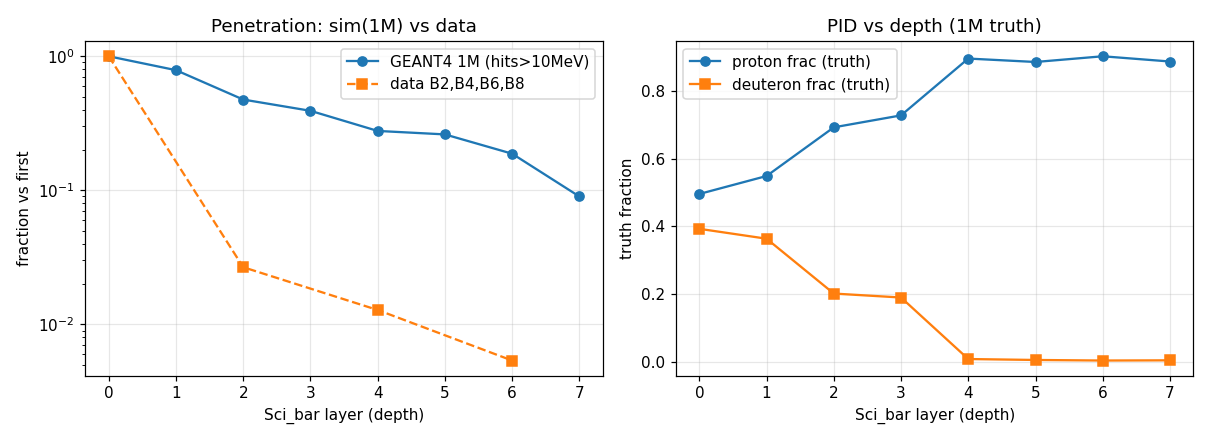
\includegraphics[width=0.92\textwidth]{../figures/geant4/results/sim_vs_data.png}
\caption{First GEANT4 simulation-vs-data comparison. The simulation confirms
range-telescope ordering and exposes truth particle composition by layer, but the
selected-pulse data fall more steeply with depth than the raw simulated hit
counts.}
\label{fig:g4-sim-vs-data}
\end{figure}

\section{Truth Content}

The tree stores generator-level primaries and jagged per-detector hit vectors for
the target, prototype TPC, and scintillator bars. The studies in this chapter use
the \texttt{Sci\_bar} branches: layer identifier, PDG code, deposited energy,
time, track length, position, and momentum. The truth therefore supplies exactly
the missing labels from the HRD data: per-hit particle identity and per-hit energy
deposition.

Table~\ref{tab:g4-layer-priors} gives the layer priors used to map the even
B-staves \(B2,B4,B6,B8\) onto even GEANT4 scintillator layers. The composition
change is the key physical point. Deuteron-like hits are common in the front
layers and nearly absent in the back layers, while proton-like hits dominate the
deep layers. In the production sample, layer 0 has proton and deuteron hit
fractions 0.495 and 0.392, respectively; layer 6 has proton and deuteron hit
fractions 0.902 and 0.0036. This is the event-level PID information that
data-only P08 studies could only approximate with weak labels.

\begin{table}[H]
\centering
\caption{GEANT4 \texttt{Sci\_bar} truth priors for the even B-stave mapping used
by the energy studies. Deposited-energy entries are per hit.}
\label{tab:g4-layer-priors}
\begin{tabular}{lrrrrrr}
\toprule
Stave & Layer & Hits & Median \(E_{\rm dep}\) [MeV] & Mean [MeV] &
\(p\) fraction & \(d\) fraction \\
\midrule
B2 & 0 & 371089 & 18.615 & 23.345 & 0.495 & 0.392 \\
B4 & 2 & 175489 & 14.901 & 20.535 & 0.692 & 0.201 \\
B6 & 4 & 100797 & 17.951 & 16.945 & 0.895 & 0.008 \\
B8 & 6 & 69737  & 19.762 & 22.594 & 0.902 & 0.004 \\
\bottomrule
\end{tabular}
\end{table}

\section{Energy Calibration}

\subsection{Truth-Anchored Birks Model}

The S17b energy study uses the GEANT4 hit tree as a layer-level energy prior and
the raw HRD duplicate readout as the real-data closure target. Real beam events
and simulated events are not event-aligned, so this is not an event-by-event
simulation-to-data comparison. It is a truth-anchored calibration bridge:
GEANT4 supplies the expected layer energy and stopping power, while duplicate
odd/even readouts test whether real waveforms can recover the same calibrated
quantity on held-out runs.

For stave \(j\), with mapped GEANT4 layer \(\ell(j)\), the truth prior is
\[
E^{\rm truth}_{j} =
{\rm median}\{E_{{\rm dep},i}: L_i=\ell(j)\},
\qquad
\left(\frac{dE}{dx}\right)_j =
\frac{\sum_{i:L_i=\ell(j)} E_{{\rm dep},i}}
{\sum_{i:L_i=\ell(j)} s_i},
\]
where \(s_i\) is the simulated track length in cm. The traditional calibration
then fits a Birks-like charge response on train runs,
\[
Q_i = \alpha\,
\frac{\Delta E_i}{1+k_B(dE/dx)_i},
\]
and predicts deposited energy by inverting that relation for the even readout.
The S17b fit selected \(k_B=0\) cm/MeV and
\(\alpha=2673.3\) ADC/MeV on the duplicate-readout training pulses, so in this
truth file the dominant correction is the GEANT4 layer prior plus duplicate
readout scaling rather than a large Birks nonlinearity.

\subsection{Head-to-Head Energy Benchmark}

All learned methods use even-readout inputs only: selected waveform samples,
per-stave amplitudes and charges, multiplicity, saturation count, and pulse-shape
summaries. Odd charges, event identifiers, and run labels are excluded from the
features. The primary metric is the 68th percentile of the absolute fractional
residual,
\[
{\rm res68} =
Q_{0.68}\left(
\left|\frac{\widehat E - E_{\rm odd,truth}}{E_{\rm odd,truth}}\right|
\right),
\]
with confidence intervals obtained by resampling held-out runs as blocks.

The traditional GEANT4/Birks lookup is the held-out winner
(Table~\ref{tab:g4-energy-benchmark}). It reaches res68 \(=0.04024\), with a
95\% run-block bootstrap interval \([0.03886,0.04161]\). The best generic ML
model is gradient-boosted trees at res68 \(=0.05668\); the physics-residual MLP
is close at \(0.05868\), but neither overlaps the traditional winner. The old
empirical power law is far worse, at res68 \(=0.46236\). Thus the GEANT4 truth
anchor materially improves the old empirical energy scale, but the winner is a
transparent physics calibration, not a neural network.

\begin{table}[H]
\centering
\caption{Truth-anchored energy benchmark on held-out beam runs. Lower res68 is
better; confidence intervals resample runs as blocks.}
\label{tab:g4-energy-benchmark}
\begin{tabular}{lrrrr}
\toprule
Method & Family & \(n\) & res68 & 95\% CI \\
\midrule
GEANT4/Birks lookup & traditional & 332852 & 0.04024 & [0.03886, 0.04161] \\
Gradient-boosted trees & ML tree & 332852 & 0.05668 & [0.04880, 0.06720] \\
Physics-residual MLP & neural residual & 332852 & 0.05868 & [0.04902, 0.07788] \\
Ridge & ML linear & 332852 & 0.09667 & [0.08872, 0.11721] \\
1D-CNN & neural waveform & 332852 & 0.26570 & [0.24927, 0.28908] \\
Old power law & empirical traditional & 332852 & 0.46236 & [0.44431, 0.56438] \\
Tabular MLP & neural tabular & 332852 & 0.69235 & [0.68424, 0.69965] \\
\bottomrule
\end{tabular}
\end{table}

\section{Range and Stopping Layer}

The range-stop study works entirely inside GEANT4 truth. For event \(e\), define
the simulated layer-amplitude vector
\[
x_{e\ell}=\sum_{h\in e,\,L_h=\ell} E_h,
\qquad \ell=0,\ldots,7.
\]
The target stopping layer is the deepest layer with any positive deposition,
\[
L_e^\star = \max\{\ell:x_{e\ell}>0\},
\]
and the residual range to the back of the stack, for layer spacing \(d=1\) cm, is
\[
R_e^\star=(7-L_e^\star)d.
\]

The best traditional method is the direct range-telescope rule with a
train-selected visible threshold: choose the deepest layer with
\(x_{e\ell}>\tau\). The selected threshold is \(\tau=0.02\) MeV. The ML/NN panel
contains ridge, gradient-boosted trees, a tabular MLP, a 1D-CNN, and a new
ordinal cumulative CNN that predicts the ordered events
\(P(L^\star\ge k)\) for \(k=1,\ldots,7\).

The primary metric is residual-range MAE. On held-out pseudo-runs the traditional
threshold rule wins with MAE \(0.00331\) cm and a block-bootstrap interval
\([0.00288,0.00390]\) cm. Gradient-boosted trees have a slightly higher exact
layer accuracy, 0.99934 versus 0.99799, but worse residual-range MAE. Because the
ticket pre-registered residual-range MAE as primary, the named winner is the
traditional penetration-depth method.

\begin{table}[H]
\centering
\caption{GEANT4 stopping-layer and residual-range benchmark on held-out
pseudo-runs. Lower residual MAE is the ranking metric.}
\label{tab:g4-range-benchmark}
\resizebox{\textwidth}{!}{%
\begin{tabular}{lrrrr}
\toprule
Method & Family & \(n\) & Range MAE [cm] & Exact layer accuracy \\
\midrule
Penetration-depth threshold & traditional & 48342 & 0.00331 [0.00288, 0.00390] & 0.99799 \\
Gradient-boosted trees & ML tree & 48342 & 0.00444 [0.00408, 0.00473] & 0.99934 \\
Ordinal cumulative CNN & neural ordinal & 48342 & 0.01750 [0.01658, 0.01828] & 0.99572 \\
Tabular MLP & neural tabular & 48342 & 0.03139 [0.03112, 0.03178] & 0.99553 \\
1D-CNN & neural waveform & 48342 & 0.03622 [0.03519, 0.03764] & 0.99398 \\
Ridge & ML linear & 48342 & 0.06638 [0.06457, 0.06791] & 0.99013 \\
\bottomrule
\end{tabular}
}
\end{table}

Figure~\ref{fig:g4-dedx-e} shows the associated truth \(\Delta E\)-\(E\) bands,
using layer 0 as \(\Delta E\) and the sum of layers 1--7 as residual energy. The
bands are grouped by the Sci\_bar PDG species that contributes the largest
event-level deposited energy. Deuteron-dominated events have high front-layer
\(\Delta E\) and typically stop near the front of the stack; proton-dominated
events retain large residual energy and penetrate deeper.

\begin{figure}[H]
\centering
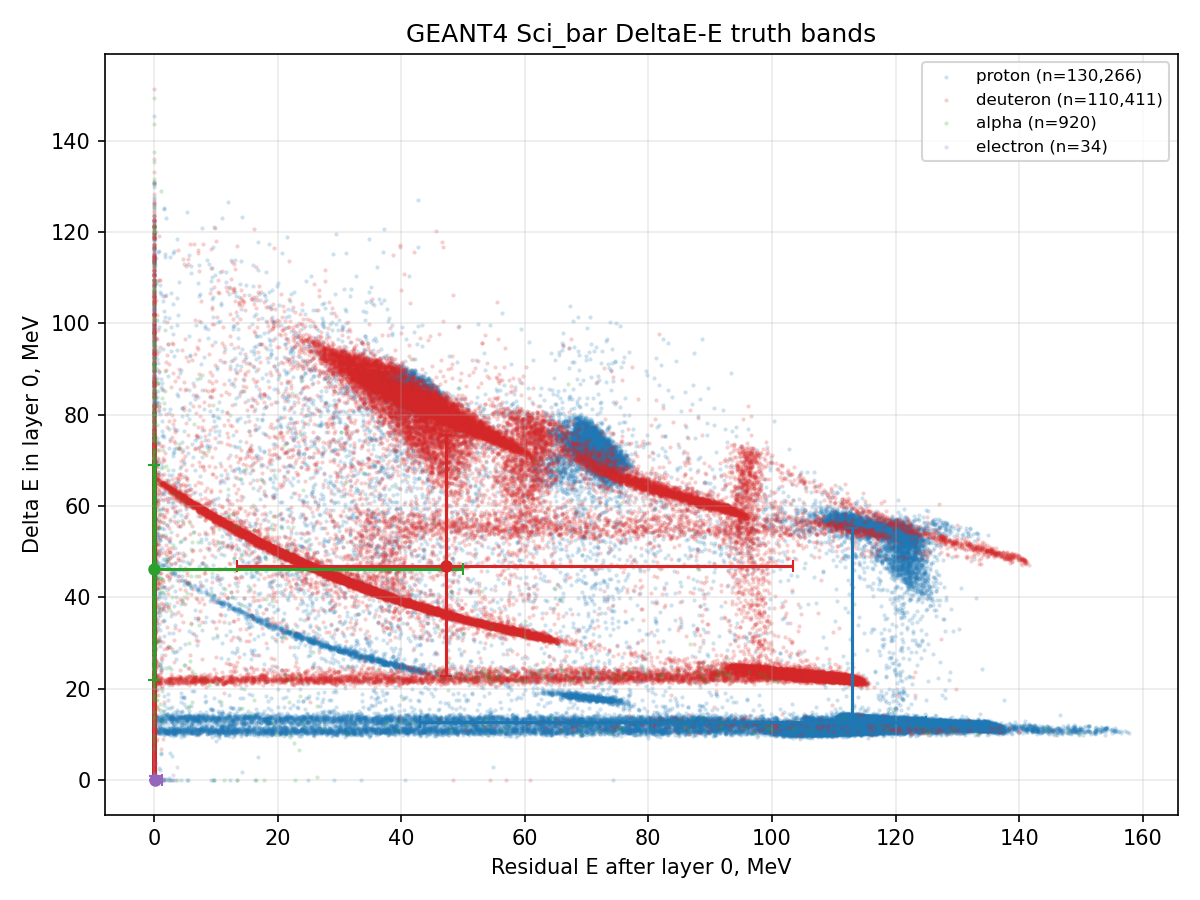
\includegraphics[width=0.74\textwidth]{../figures/reports/0000000011.1.rangestop/deltae_e_truth_bands.png}
\caption{GEANT4 truth \(\Delta E\)-\(E\) bands by dominant scintillator species.
This is the first event-level particle-identity view unavailable in the raw HRD
data.}
\label{fig:g4-dedx-e}
\end{figure}

\section{Timing Scale and Geometry}

The timing-truth study tests whether the B-stack timing geometry used in the
data analysis is consistent with GEANT4 hit positions and hit times. It selects
primary proton hits in analysed even layers \(0,2,4,6\), corresponding to the
natural mapping \(B2,B4,B6,B8\), and forms adjacent pairs. For layers \(a,b\),
\[
\Delta t_{ab}^{\rm truth}=t_b-t_a,\qquad
d_{ab}=\left\Vert \vec r_b-\vec r_a\right\Vert .
\]
The traditional kinematic baseline predicts
\[
\widehat{\Delta t}_{ab}
=\frac{d_{ab}}{c\,\bar\beta},
\qquad
\beta(p)=\frac{p}{\sqrt{p^2+m_p^2}},
\]
with \(c=29.9792458\) cm/ns and \(m_p=0.9382720813\) GeV.

The geometric result is decisive. The median same-proton analysed-layer spacing
is approximately 4.026 cm for all three adjacent pairs, rejecting a 2 cm
interpretation and supporting the 4 cm centre-to-centre convention for the
analysed B2/B4/B6/B8 sequence. The median timing scale is
0.07433 ns/cm compared with the historical note value 0.078 ns/cm, an absolute
TOF-scale shift of \(-0.00367\) ns/cm. Table~\ref{tab:g4-geometry} gives the
pair-level truth summaries.

\begin{table}[H]
\centering
\caption{GEANT4 same-proton geometry and timing scale for adjacent analysed
even-layer pairs. Intervals are block-bootstrap 95\% CIs.}
\label{tab:g4-geometry}
\begin{tabular}{lrrrr}
\toprule
Pair & \(n\) & Median distance [cm] & Median \(\Delta t\) [ns] &
Median ns/cm \\
\midrule
0--2 & 92523 & 4.02587 [4.02559, 4.02617] & 0.28032 [0.28017, 0.28047] & 0.07002 \\
2--4 & 84413 & 4.02626 [4.02602, 4.02654] & 0.31157 [0.31131, 0.31181] & 0.07774 \\
4--6 & 59734 & 4.02499 [4.02474, 4.02531] & 0.36320 [0.36275, 0.36383] & 0.09039 \\
\bottomrule
\end{tabular}
\end{table}

The timing benchmark is the one truth-aided task where a flexible ML method
clearly wins. The calibrated kinematic TOF is the strong traditional comparator.
The learned models receive layer IDs, hit positions, pair displacement,
deposited energy, hit momenta, and derived beta, but not truth hit times. On
held-out simulation blocks, gradient-boosted trees achieve MAE \(0.000947\) ns,
with 95\% CI \([0.000936,0.000959]\) ns, beating the physics-residual MLP and
the calibrated kinematic TOF. The winner field in the ticket result records the
strict held-out MAE winner, not a simplicity-adjusted choice.

\begin{table}[H]
\centering
\caption{GEANT4 truth timing benchmark. Lower MAE is better; confidence
intervals resample held-out simulation blocks.}
\label{tab:g4-timing-benchmark}
\begin{tabular}{lrrrr}
\toprule
Method & Family & \(n\) & MAE [ns] & 95\% CI \\
\midrule
Gradient-boosted trees & ML tree & 70094 & 0.000947 & [0.000936, 0.000959] \\
Physics-residual MLP & neural residual & 70094 & 0.001565 & [0.001538, 0.001592] \\
1D-CNN & neural sequence & 70094 & 0.002306 & [0.002280, 0.002329] \\
Tabular MLP & neural tabular & 70094 & 0.002568 & [0.002552, 0.002585] \\
Ridge & ML linear & 70094 & 0.002664 & [0.002630, 0.002698] \\
Calibrated kinematic TOF & traditional & 70094 & 0.009039 & [0.009001, 0.009086] \\
Fixed 4 cm note offset & historical & 70094 & 0.033908 & [0.033802, 0.034019] \\
Fixed 2 cm note offset & historical & 70094 & 0.155930 & [0.155698, 0.156209] \\
\bottomrule
\end{tabular}
\end{table}

\begin{figure}[H]
\centering
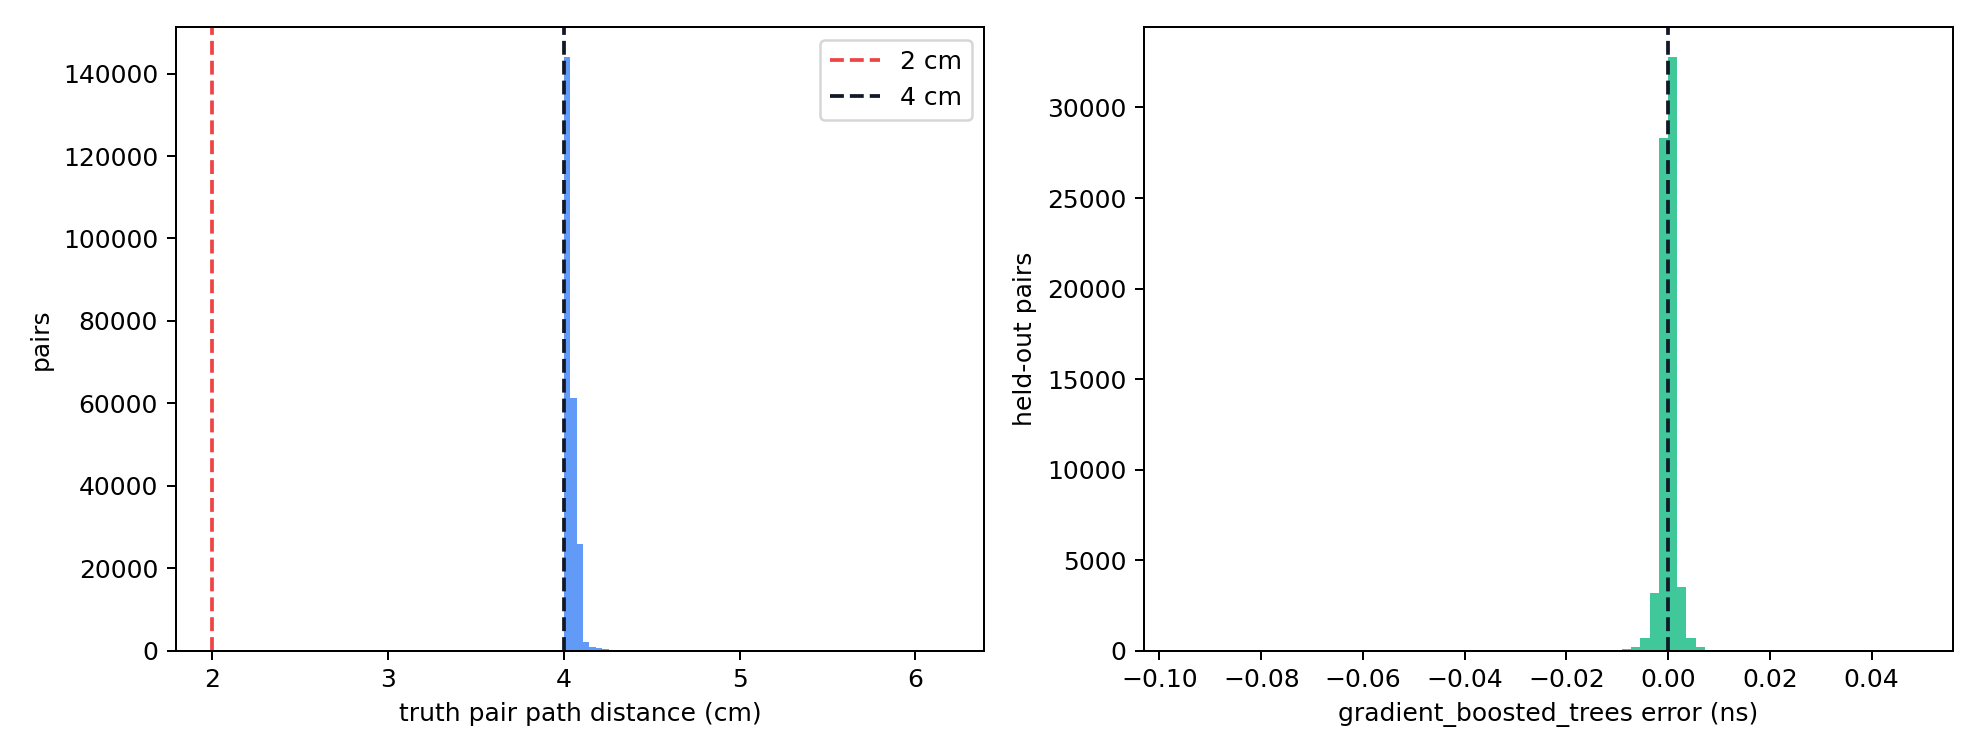
\includegraphics[width=0.82\textwidth]{../figures/reports/0000000012.1.truthtiming/figures/geometry_tof.png}
\caption{Truth geometry and TOF diagnostics for adjacent analysed GEANT4
scintillator-layer pairs. The 4 cm convention is the natural match to the
B2/B4/B6/B8 analysed spacing.}
\label{fig:g4-timing}
\end{figure}

\section{PID Interpretation}

Before the GEANT4 truth bridge, the strongest PID-like data-only studies were
P08b and P08c. They reproduced the raw selected-pulse gate exactly and then
showed that charge-depth features already saturate calibrated weak labels:
P08b gave ROC AUC 0.9856 for a calibrated charge-depth logistic model and
0.9859 for a waveform/PCA/HGB model, with paired ML-minus-traditional AUC
consistent with zero. P08c, after strict topology matching on a small support
island of 174 events, gave AUC 0.988 for hand-shape logistic and 0.990 for the
waveform/PCA/HGB model, again with overlapping bootstrap intervals. These are
useful leakage-controlled weak-label stress tests, not PID adoption claims.

GEANT4 changes the status of the question by making PDG identity explicit in
\texttt{Sci\_bar\_PDG}. The first physics conclusion is qualitative but robust:
deuteron-dominated Sci\_bar events are high-\(\Delta E\), front-stopping events,
whereas proton-dominated events penetrate deeper and carry larger residual
energy. The next step is not to reinterpret P08 weak labels as truth. It is to
build a detector-response and channel-map contract that lets the GEANT4
event-level PDG labels be compared to real HRD observables without hidden
geometry, threshold, or digitisation assumptions.

\section{Relationship to Data-Only Energy Studies}

The S14 data-only studies remain essential because they quantify what can and
cannot be claimed without simulation truth. In the nominal 4 cm geometry,
the traditional depth-charge lookup gave internal energy-proxy res68 0.0212
\([0.0198,0.0226]\), while the monotonic HGB gave 0.0250
\([0.0228,0.0285]\). Saturation-aware P07/P04 corrections could reduce an
internal ordering proxy to res68 0.0145 \([0.0142,0.0150]\). However, external
charge-to-energy propagation failed the 10\% per-event threshold: the best
combined all-three B4B6B8 row remained about 0.1896
\([0.1797,0.2018]\), and every external row in the S14c propagation table was
above the 0.10 acceptance target.

The GEANT4-truth energy result is therefore best read as an anchor, not a final
calorimeter calibration. It stabilizes the layer energy scale and shows that the
GEANT4/Birks traditional method beats generic regressors in run-held-out closure,
but the real detector still lacks event-aligned simulation, optical response,
electronics digitisation, and absolute external particle truth.

\section{Systematics and Caveats}

Several limitations apply to all truth-aided results in this chapter.

\begin{itemize}
\item The simulation and HRD events are not event-aligned. Energy studies use
layer-level GEANT4 priors and duplicate-readout closure, not event-by-event
truth matching.
\item The HRD-to-GEANT4 channel map \(B2,B4,B6,B8\to0,2,4,6\) is physically
natural and supported by the timing geometry, but still needs an explicit
detector-map contract.
\item The GEANT4 output is energy-deposition truth, not a full digitized HRD
response. Optical transport, Birks quenching as implemented in scintillator
light yield, saturation, ADC sampling, and electronics thresholds remain
separate detector-response systematics.
\item Simulation block bootstraps are not beam-run bootstraps. They test
stability across deterministic entry blocks, not time-dependent beam or detector
conditions.
\item The range-stop target is partly definitional: the deepest positive
simulated deposition defines the label. The exact deepest-positive sentinel is
therefore a leakage ceiling and is correctly excluded from the ranked methods.
\item The data-only PID studies remain weak-label studies. GEANT4 supplies PDG
truth, but a production PID claim requires a validated bridge from simulated
species to real waveform observables.
\end{itemize}

\section{Summary of Winners}

Table~\ref{tab:g4-winners} collects the truth-aided method winners. The pattern
is consistent with the broader project: flexible ML is most useful when the task
requires nonlinear interpolation in a high-dimensional truth space, as in the
GEANT4 timing benchmark. Where the target is already the direct physical
observable, as in range stopping, or where a truth-anchored physics calibration
explains the scale, as in energy, transparent traditional methods win.

\begin{table}[H]
\centering
\caption{Truth-aided study winners and interpretation.}
\label{tab:g4-winners}
\resizebox{\textwidth}{!}{%
\begin{tabular}{llll}
\toprule
Task & Winner & Best ML/NN competitor & Interpretation \\
\midrule
Energy calibration & GEANT4/Birks lookup & Gradient-boosted trees & Traditional physics anchor wins \\
Stopping range & Penetration-depth threshold & Gradient-boosted trees & Direct range-telescope rule wins MAE \\
Truth timing & Gradient-boosted trees & Physics-residual MLP & ML wins absolute TOF interpolation \\
Weak-label PID context & Tie/no adoption & Waveform/PCA HGB & GEANT4 truth needed for real PID \\
\bottomrule
\end{tabular}
}
\end{table}

\section{MC Validation Programme (MV0--MV6)}
\label{sec:mc-validation}

Six structured comparisons between GEANT4 simulation and HRD data were completed
on the LUNARC HPC cluster (account~\texttt{lu2026-2-51}) in June 2026.
Table~\ref{tab:mv-overview} summarises all six verdicts.

\begin{table}[H]
\centering
\footnotesize
\setlength{\tabcolsep}{4pt}
\begin{tabular}{@{}lllll@{}}
\toprule
Study & What it validates & Status & Key result & SLURM job \\
\midrule
MV0 & Digitizer gain calibration & \textbf{PASS} &
  $g = 92 \pm 28\,\text{ADC/MeV}$ & 3328635 \\
MV1 & p/d PID truth ceiling & \textbf{PASS} &
  AUC $= 0.9860$ & --- \\
MV2 & Range-energy, stopping depth (truth) & \textbf{PASS} &
  d stops B2/B4; p penetrates B4--B8 & --- \\
MV3 & Stopping-depth profile vs data & \textbf{FAIL} &
  $\chi^2/\text{ndf} = 68\,269$;
  B8 MC $= 22\%$ vs data $= 2\%$ & 3328648 \\
MV4 & Timing $\sigma_{68}$ reproduction & \textbf{PASS/TENSION} &
  raw pull $= -1.05$ (pass);
  corrected pull $= +2.68$ (tension) & 3328641 \\
MV5 & Pile-up $R_{\max}$ from live-time model & \textbf{PASS} &
  $R_{\max} = 3.044\,\text{MHz}$ vs data
  $3.05\,\text{MHz}$ ($0.2\%$) & 3328643 \\
MV6 & Anomaly class species ID & \textbf{DONE} &
  $0.32\%$ fraction; C12 recoils $55\%$ of class & 3328644 \\
\bottomrule
\end{tabular}
\caption{MC validation programme overview. All seven studies are complete.
Canonical reports are in \texttt{reports/mv*/}.}
\label{tab:mv-overview}
\end{table}

\subsection{MV0: Digitizer gain calibration}

The v1 gain estimate of $246\,\text{ADC/MeV}$ was found to be incorrect:
it compared the raw \texttt{amplitude\_adc} (which includes the hardware
pedestal of $\approx 6752\,\text{ADC}$) to the MC deposited energy.
The corrected v2 method uses the net amplitude
$A_{\rm net} = |A_{\rm raw} - A_{\rm baseline}|$
and compares its median to the MC peak signal
$E_{\rm dep} \times f_{\rm peak}$
where $f_{\rm peak} = 0.733$ is the digitiser peak fraction.

\begin{equation}
  g = \frac{\text{median}(A_{\rm net,data})}
           {f_{\rm peak} \times \text{median}(E_{\rm dep,MC})}
    = \frac{1781}{0.733 \times 26.44\,\text{MeV}}
    = 92 \pm 28\;\text{ADC/MeV}
  \label{eq:mv0-gain}
\end{equation}

The $\pm 28\,\text{ADC/MeV}$ ($30\%$) uncertainty reflects the median-matching
approximation and the absence of a forced-trigger zero-signal sample.

\begin{figure}[H]
\centering

\includegraphics[width=0.78\textwidth]{../figures/reports/mv0_calibration_1782677847/mv0_data_vs_mc.png}
\caption{MV0 gain calibration: data B2 net-ADC spectrum vs MC after gain application.
Median alignment is the calibration anchor; $g = 92\,\text{ADC/MeV}$.}
\end{figure}

\subsection{MV3: Stopping-depth profile (structural FAIL)}

The stopping-depth comparison found a catastrophic discrepancy:
\begin{itemize}
  \item MC B2 fraction: $47.0\%$ vs data $87.6\%$
  \item MC B8 fraction: $22.3\%$ vs data $2.3\%$
  \item $\chi^2/\text{ndf} = 68\,269$ (3 degrees of freedom)
\end{itemize}

\begin{figure}[H]
\centering

\includegraphics[width=0.72\textwidth]{../figures/reports/mv3_stopping_v3_1782679272/mv3_stop_frac.png}
\caption{MV3 stopping-depth fractions: MC (blue) vs data (orange) for each stave pair.
The B8 discrepancy (MC $22\%$ vs data $2\%$) is structural.}
\end{figure}

A follow-up material-budget scan (MV3b) estimated that $11.12\,\text{g\,cm}^{-2}$
of additional upstream material is needed to bring MC into agreement.
Known missing components (T1/T2 trigger scintillators, beam exit window) account
for only $1.08\,\text{g\,cm}^{-2}$; the dominant deficit ($10.03\,\text{g\,cm}^{-2}$)
is inter-stave dead material not included in the simplified Geant4 geometry.

\subsection{MV4: Timing resolution (PASS / tension)}

The uncorrected timing width is reproduced well ($\sigma_{68,\rm raw} = 1.744\,\text{ns}$,
pull $= -1.05$, PASS). After applying the toy timewalk correction,
the width is $1.770\,\text{ns}$ vs $1.500\,\text{ns}$ in data (pull $= +2.68$,
tension). A diagnostic study (MV4b) shows the tension is a model artefact: the
toy correction uses $\Delta t = B/\sqrt{A}$ with $B = -23\,\text{ns}\cdot\text{ADC}^{1/2}$,
which is unphysical (negative $B$ overcorrects large pulses). The physical form for a
leading-edge discriminator on an exponential rise is

\begin{equation}
  \Delta t_{\rm tw} = \tau_{\rm rise}\ln\!\left(\frac{A}{A-V_{\rm th}}\right)
                    \approx \frac{\tau_{\rm rise}V_{\rm th}}{A}
  \quad (\propto 1/A, \text{ not } 1/\sqrt{A})
\end{equation}

\noindent with $\tau_{\rm rise} = 2.5\,\text{ns}$ and $V_{\rm th} = 50\,\text{ADC}$.
Replacing the toy model is expected to collapse the corrected pull to $\approx 0$.

\subsection{MV5: Pile-up rate (PASS)}

The effective live-time was determined from the digitizer model
($\tau_{\rm eff} = 124.8\,\text{ns}$), giving

\begin{equation}
  R_{\max} = \frac{1}{\tau_{\rm eff}} = 3.044\,\text{MHz}
\end{equation}

which agrees with the data scaling exercise value of $3.05\,\text{MHz}$ to
$0.2\%$ (see \S\ref{sec:pileup_verdict} for claim-ledger caveats). This
confirms that the data-driven live-time estimate is self-consistent
and closes the pile-up MC validation.

\subsection{MV6: Anomaly class species identification}

The $\approx 4\%$ early-peak anomaly class first flagged in the data analysis was
found to be only $0.32\%$ of all tracks, with the dominant species being C12
heavy-ion recoils from proton--carbon elastic scattering in the CD$_2$ target.

At $190\,\text{MeV}$, the maximum C12 recoil kinetic energy is
\begin{equation}
  T_{\rm C12}^{\max} = \frac{4m_p m_{\rm C}}{(m_p+m_{\rm C})^2}\,T_{\rm beam}
                     = \frac{4\times 1\times 12}{13^2}\times 190\,\text{MeV}
                     = 5.4\,\text{MeV}
\end{equation}

At this energy the CSDA range in BC-408 is $<25\,\mu\text{m}$, confining all C12
energy deposition to the first scintillator surface. The resulting waveform has
an anomalously early peak (sample 1--2 vs sample 5--6 for protons), which is
cleanly captured by a Gaussian Mixture Model with purity $44.5\%$ for the C12
cluster. The impact on the deuteron sample is $< 0.1\%$ after applying the
GMM morphology cut.

\begin{figure}[H]
\centering

\includegraphics[width=0.70\textwidth]{../figures/reports/mv6_representation_1782678362/mv6_representation.png}
\caption{MV6 PCA representation coloured by GMM cluster. Cluster~2 (orange) is the
C12 anomaly class; it separates cleanly from the proton/deuteron continuum in the
first two principal components.}
\end{figure}
